% Copyright (c)  2005-2010 EDF-EADS-PHIMECA.
% Permission is granted to copy, distribute and/or modify this document
% under the terms of the GNU Free Documentation License, Version 1.2
% or any later version published by the Free Software Foundation;
% with no Invariant Sections, no Front-Cover Texts, and no Back-Cover
% Texts.  A copy of the license is included in the section entitled "GNU
% Free Documentation License".
\renewcommand{\etapemethodo}{B}
\renewcommand{\nomfichier}{docref_B122_RandomMixture}
\renewcommand{\titrefiche}{Random Mixture : affine combination of independent univariate distributions}

\Header

\MathematicalDescription{

  \underline{\textbf{Goal}}\vspace{2mm}

  One univariate random variable may be defined as an affine combination of independent univariate random variable, as follows :
  \begin{equation}
    \displaystyle Y = a_0 + \sum_k a_k X_k
    \label{RandomMixtureFormula}
  \end{equation}
  where $(a_i)_{ 0 \leq k \leq n} \in \mathbb{R}$ and $(X_k)_{ 1 \leq k \leq n}$ are some independent univariate distributions.\\

  In such a case, it is possible to evaluate directly the distribution of $Y$ and then to ask $Y$ any request compatible with a distribution : moments, quantiles, probability and cumulative density functions ...
  \vspace*{2mm}




  \underline{\textbf{Principle}}
  \vspace*{2mmm}

  {\bf Evaluation of the probability density  function of the Random Mixture}

  As the univariate random variables $X_i$ are independent, the  characteristic function of $Y$, denoted $\phi_Y$, is easily defined from the characteristic function of $X_k$ denoted $\phi_{X_k}$ as follows :
  \begin{equation}
    \displaystyle \phi_Y(u) = e^{ia_0u} \prod_k \phi_{X_k} (a_ku), \mbox{  for } u \in \mathbb{R}
    \label{CharactFuncY}
  \end{equation}

  Once $ \phi_Y$ evaluated, it is possible to evaluate the probability density  function of $Y$, denoted $p_Y$ : several techniques are possible, as the inversion of the Fourier transformation. This technique is not easy to implement.\\
  Open TURNS uses another technique, based on the Poisson sum formulation, defined as follows :
  \begin{equation}
    \displaystyle   \sum_{k \in \mathbb{Z}} p_Y(y+\frac{2k\pi}{h}) = \frac{h}{2\pi}\sum_{k \in \mathbb{Z}}  \phi_Y(kh)e^{-ikhy}
    \label{PoissonSum}
  \end{equation}

  If $h \approx 0$, then  $\frac{2k\pi}{h} \approx +\infty$ and $p_Y(y+\frac{2k\pi}{h})  \approx 0$ because of the decreasing properties of $p_Y$. Thus, for $h$ \emph{little enough}, the left term of (\ref{PoissonSum}) is approximatively equal to $p_Y(y)$.\\
  Furthermore, the right term of (\ref{PoissonSum}) is a series which converges very fast: only few terms of the series are enough to get machine-precision accuracy. Let us note that the factors $\phi_Y(kh)$, which are expensive to evaluate, do not depend on $y$ and are evaluated once only.\\
  \vspace*{2mm}

  {\bf Evaluation of the moments of the Random Mixture}

  The relation (\ref{RandomMixtureFormula}) enables to evaluate all the moments of the random mixture, if mathematically defined. For example, we have :
  $$
  \left\{
    \begin{array}{lcl}
      E[Y] & = & a_0 + \sum_k a_k E[X_k] \\
      Var[Y] & = &  \sum_k a_k^2 Var[X_k]
    \end{array}
  \right.
  $$


  {\bf Open TURNS}\\
  In the 0.13 version of Open TURNS, distributions which are able to evaluate their characteristic function are the following ones :  $\chi^2$, Exponential, Gamma,  Laplace, Logistic, Mixture, univariate Normal, Rayleigh, Triangular, univariate TruncatedNormal, Uniform, KernelMixture (which the distribution coming from a kernel smoothing method without treatment of bounds), RandomMixture.\\
  Thus, all the requests to $Y$ that require the evaluation of the probability density function may be satisfied only if the univariate random variables $X_i$ follow distributions which characteristic function has been implemented.\\

  For all the other requests, no restriction is assigned.
}
{
  --
}


\Methodology{
  Within the global methodology, random mixtures may be used to define the output variable of interest from some indepedent univariate random variables, within the step B.
}
{
  --
}


\Example{
  The example here is an output variable of interest defined as the following combination :
  $$
  Y = 2 + 5X_1 + X_2
  $$
  where $X_1$ and $X_2$ are independent and :
  \begin{itemize}
  \item  $X_1$ follows a $\mathcal{E}xponential(1.5)$,
  \item  $X_2$ follows a $\mathcal{N}ormal(4,1)$.
  \end{itemize}

  The pdf and cdf graphs are the following ones.

  \begin{center}
    \begin{tabular}{cc}
      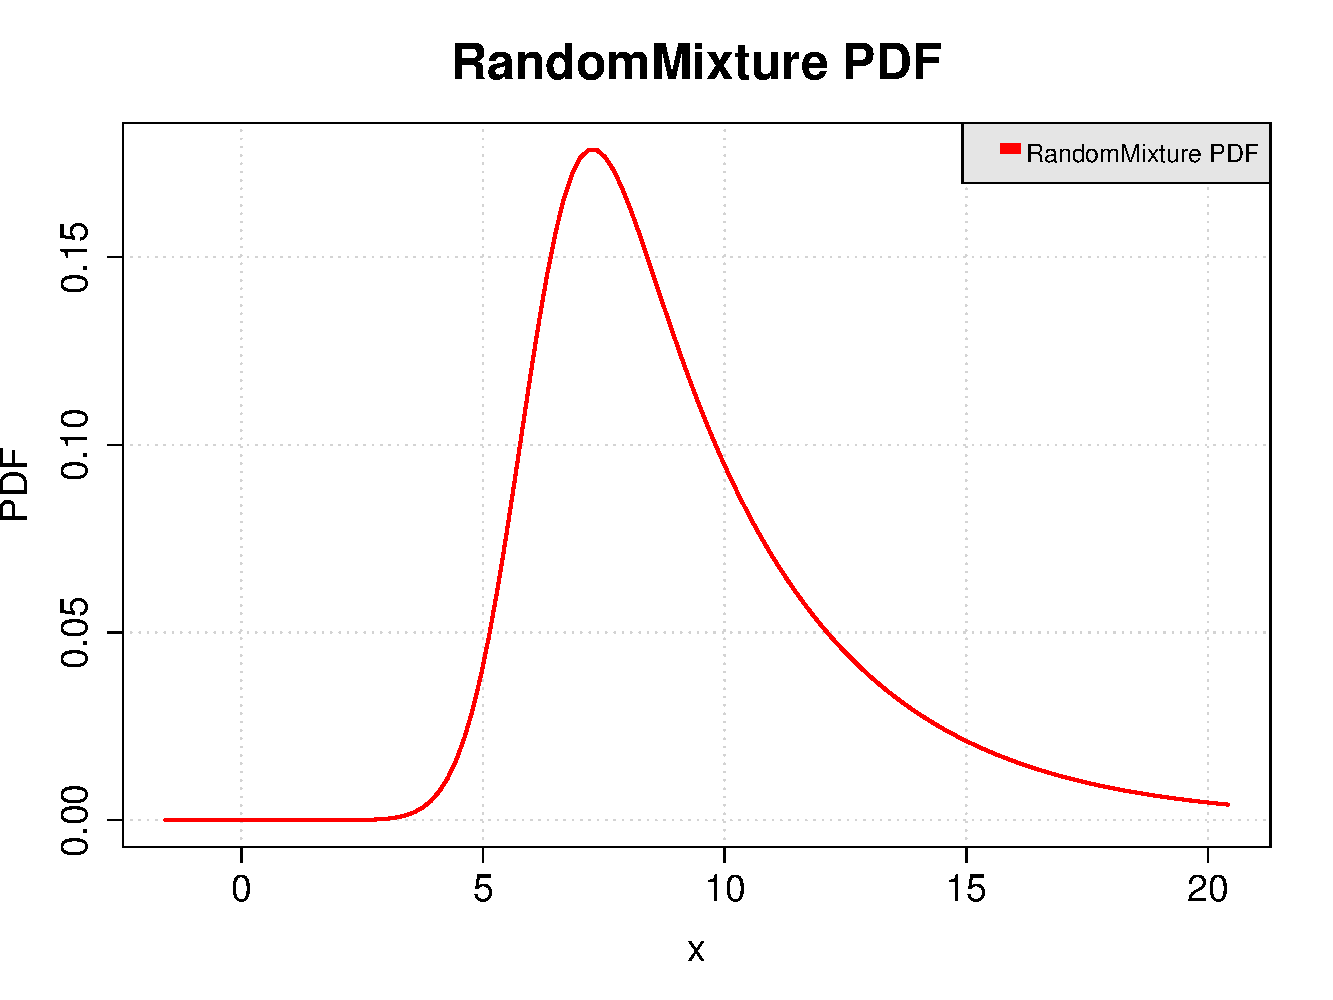
\includegraphics[width=8cm]{RandomMixture_pdf.pdf} &   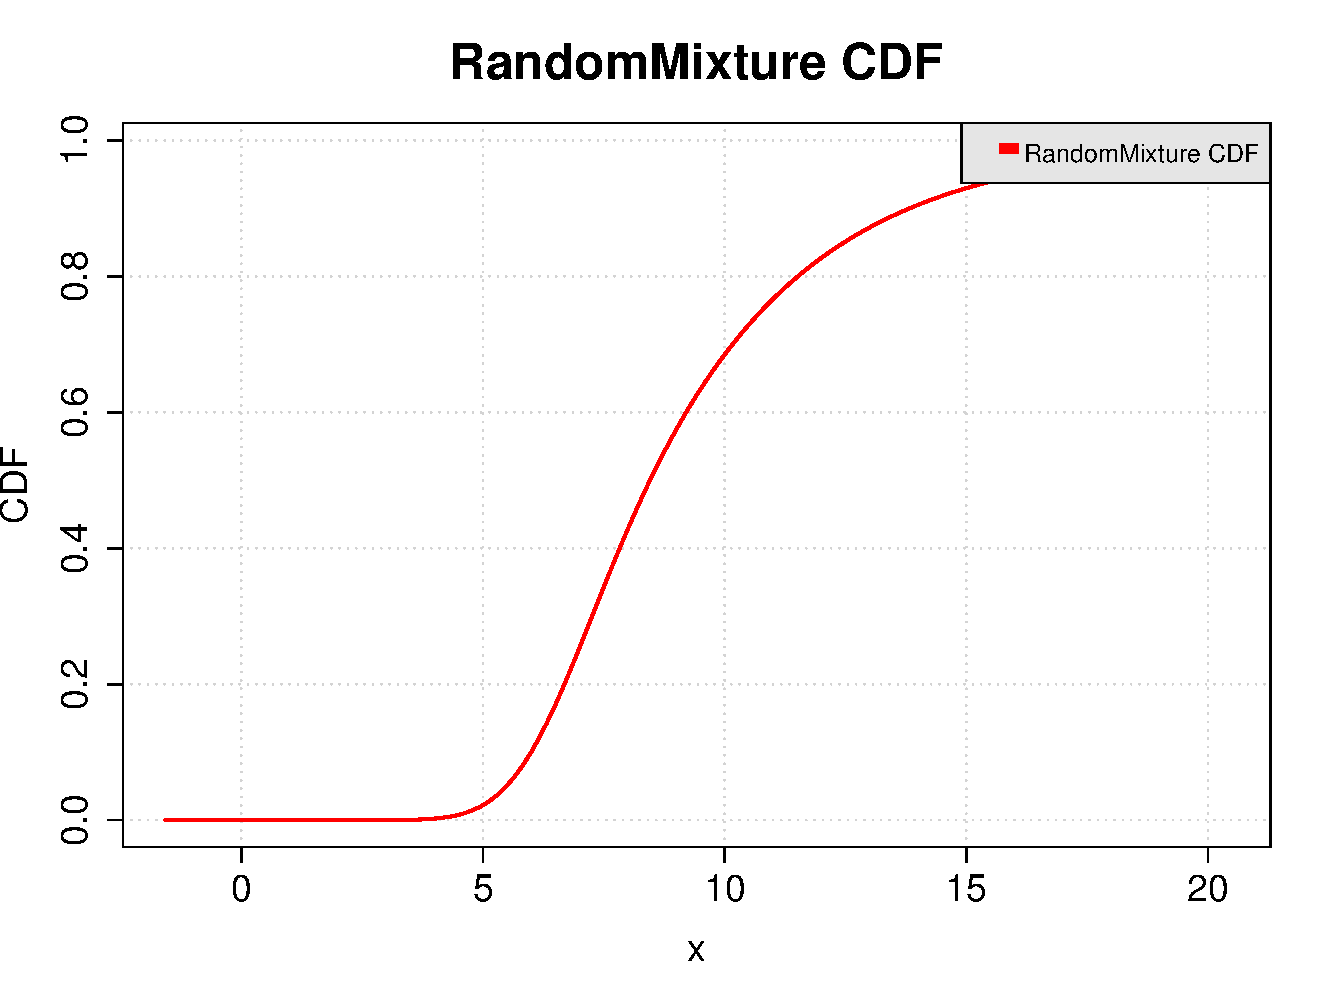
\includegraphics[width=8cm]{RandomMixture_cdf.pdf}
    \end{tabular}
  \end{center}





}
